\documentclass{standalone}
\usepackage{tikz}
\usetikzlibrary{patterns, positioning}
\usepackage[sfdefault]{ClearSans} %% option 'sfdefault' activates Clear Sans as the default text font
\usepackage[T1]{fontenc}

\begin{document}
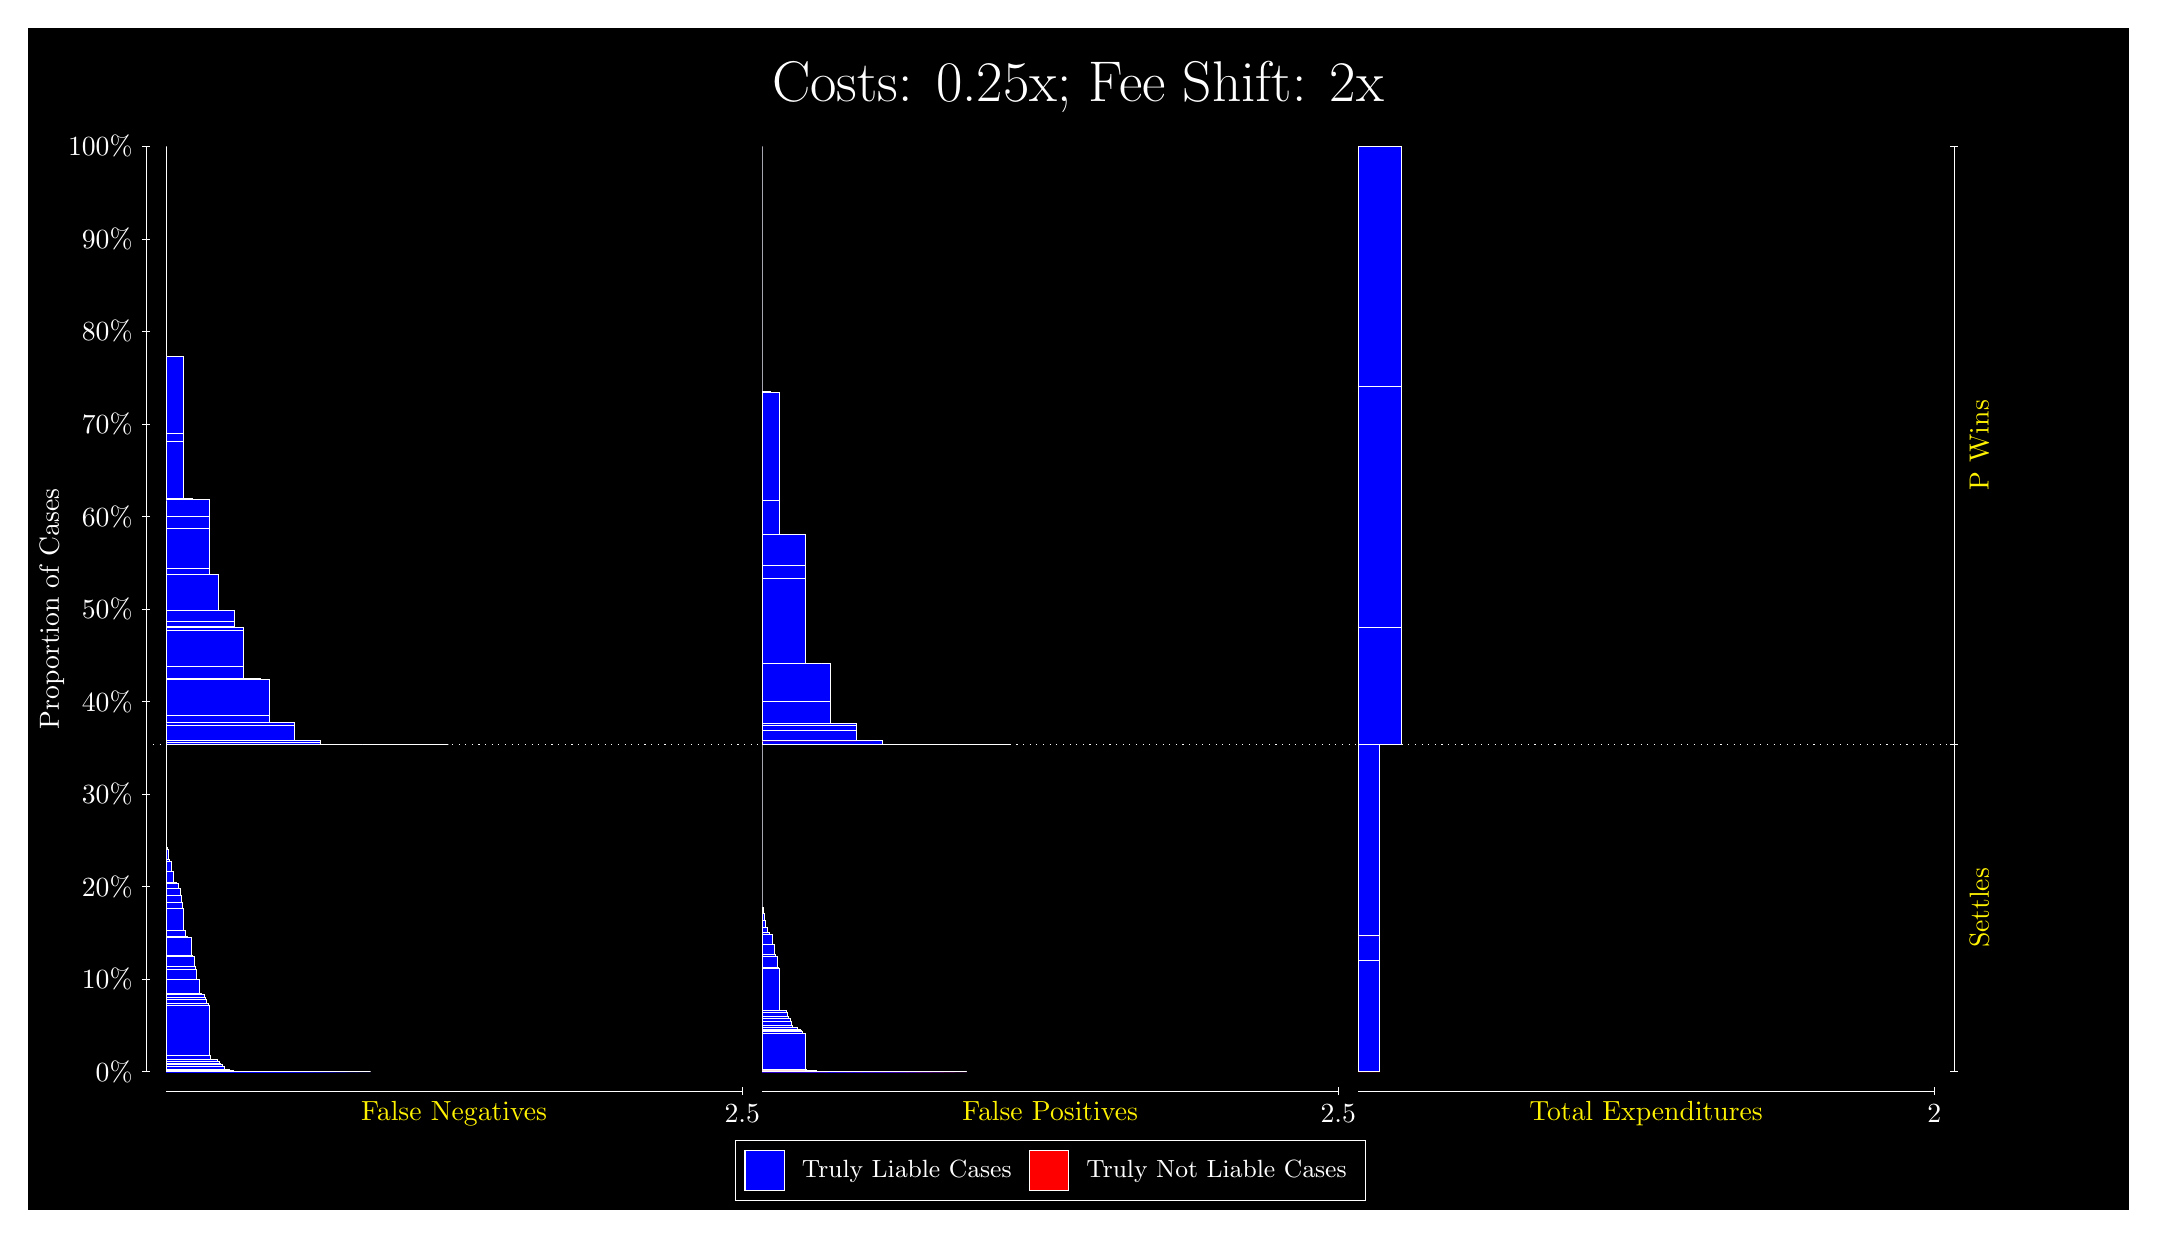
\begin{tikzpicture}
\draw[fill=black] (0,0) rectangle (26.667,15);
\draw[text=white] (0,13.5) rectangle (26.667,15) node[midway] {\huge Costs: 0.25x; Fee Shift: 2x};
\draw[white, very thin] (1.5,1.75) -- (1.5,13.5);
\node[rotate=90, text=white, anchor=center] at (0.3, 7.625) {Proportion of Cases};
\draw[white, very thin] (1.45,1.75) -- (1.55,1.75);
\node[text=white, anchor=east] at (1.45, 1.75) {0\%};
\draw[white, very thin] (1.45,2.925) -- (1.55,2.925);
\node[text=white, anchor=east] at (1.45, 2.925) {10\%};
\draw[white, very thin] (1.45,4.1) -- (1.55,4.1);
\node[text=white, anchor=east] at (1.45, 4.1) {20\%};
\draw[white, very thin] (1.45,5.275) -- (1.55,5.275);
\node[text=white, anchor=east] at (1.45, 5.275) {30\%};
\draw[white, very thin] (1.45,6.45) -- (1.55,6.45);
\node[text=white, anchor=east] at (1.45, 6.45) {40\%};
\draw[white, very thin] (1.45,7.625) -- (1.55,7.625);
\node[text=white, anchor=east] at (1.45, 7.625) {50\%};
\draw[white, very thin] (1.45,8.8) -- (1.55,8.8);
\node[text=white, anchor=east] at (1.45, 8.8) {60\%};
\draw[white, very thin] (1.45,9.975) -- (1.55,9.975);
\node[text=white, anchor=east] at (1.45, 9.975) {70\%};
\draw[white, very thin] (1.45,11.15) -- (1.55,11.15);
\node[text=white, anchor=east] at (1.45, 11.15) {80\%};
\draw[white, very thin] (1.45,12.325) -- (1.55,12.325);
\node[text=white, anchor=east] at (1.45, 12.325) {90\%};
\draw[white, very thin] (1.45,13.5) -- (1.55,13.5);
\node[text=white, anchor=east] at (1.45, 13.5) {100\%};

\draw[white, very thin] (24.457,1.75) -- (24.457,13.5);
\draw[white, very thin] (24.407,1.75) -- (24.507,1.75);
\node[anchor=west] at (24.407, 1.75) {};
\draw[white, very thin] (24.407,5.9061) -- (24.507,5.9061);
\node[anchor=west] at (24.407, 5.9061) {};
\draw[white, very thin] (24.407,13.5) -- (24.507,13.5);
\node[anchor=west] at (24.407, 13.5) {};

\draw[white, very thin, fill=blue] (1.75,1.75) rectangle (4.3482,1.75);
\draw[white, very thin, fill=blue] (1.75,1.75) rectangle (4.2018,1.75);
\draw[white, very thin, fill=blue] (1.75,1.75) rectangle (4.0554,1.75);
\draw[white, very thin, fill=blue] (1.75,1.75) rectangle (4.0229,1.75);
\draw[white, very thin, fill=blue] (1.75,1.75) rectangle (3.9091,1.75);
\draw[white, very thin, fill=blue] (1.75,1.75) rectangle (3.8765,1.75);
\draw[white, very thin, fill=blue] (1.75,1.75) rectangle (3.7627,1.75);
\draw[white, very thin, fill=blue] (1.75,1.75) rectangle (3.7302,1.75);
\draw[white, very thin, fill=blue] (1.75,1.75) rectangle (3.6976,1.75);
\draw[white, very thin, fill=blue] (1.75,1.75) rectangle (3.6163,1.75);
\draw[white, very thin, fill=blue] (1.75,1.75) rectangle (3.5838,1.75);
\draw[white, very thin, fill=blue] (1.75,1.75) rectangle (3.5513,1.75);
\draw[white, very thin, fill=blue] (1.75,1.75) rectangle (3.4699,1.75);
\draw[white, very thin, fill=blue] (1.75,1.75) rectangle (3.4374,1.75);
\draw[white, very thin, fill=blue] (1.75,1.75) rectangle (3.4049,1.75);
\draw[white, very thin, fill=blue] (1.75,1.75) rectangle (3.3723,1.75);
\draw[white, very thin, fill=blue] (1.75,1.75) rectangle (3.3236,1.75);
\draw[white, very thin, fill=blue] (1.75,1.75) rectangle (3.291,1.75);
\draw[white, very thin, fill=blue] (1.75,1.75) rectangle (3.2585,1.75);
\draw[white, very thin, fill=blue] (1.75,1.75) rectangle (3.226,1.75);
\draw[white, very thin, fill=blue] (1.75,1.75) rectangle (3.1772,1.75);
\draw[white, very thin, fill=blue] (1.75,1.75) rectangle (3.1447,1.75);
\draw[white, very thin, fill=blue] (1.75,1.75) rectangle (3.1121,1.75);
\draw[white, very thin, fill=blue] (1.75,1.75) rectangle (3.0796,1.75);
\draw[white, very thin, fill=blue] (1.75,1.75) rectangle (3.0471,1.75);
\draw[white, very thin, fill=blue] (1.75,1.75) rectangle (3.0308,1.75);
\draw[white, very thin, fill=blue] (1.75,1.75) rectangle (2.9983,1.75);
\draw[white, very thin, fill=blue] (1.75,1.75) rectangle (2.9657,1.7501);
\draw[white, very thin, fill=blue] (1.75,1.7501) rectangle (2.9332,1.7501);
\draw[white, very thin, fill=blue] (1.75,1.7501) rectangle (2.9007,1.7501);
\draw[white, very thin, fill=blue] (1.75,1.7501) rectangle (2.8844,1.7502);
\draw[white, very thin, fill=blue] (1.75,1.7502) rectangle (2.8519,1.7503);
\draw[white, very thin, fill=blue] (1.75,1.7503) rectangle (2.8194,1.7524);
\draw[white, very thin, fill=blue] (1.75,1.7524) rectangle (2.7868,1.753);
\draw[white, very thin, fill=blue] (1.75,1.753) rectangle (2.7543,1.7535);
\draw[white, very thin, fill=blue] (1.75,1.7535) rectangle (2.738,1.7536);
\draw[white, very thin, fill=blue] (1.75,1.7536) rectangle (2.7218,1.7541);
\draw[white, very thin, fill=blue] (1.75,1.7541) rectangle (2.7055,1.7542);
\draw[white, very thin, fill=blue] (1.75,1.7542) rectangle (2.673,1.7543);
\draw[white, very thin, fill=blue] (1.75,1.7543) rectangle (2.6405,1.7587);
\draw[white, very thin, fill=blue] (1.75,1.7587) rectangle (2.6079,1.7606);
\draw[white, very thin, fill=blue] (1.75,1.7606) rectangle (2.5917,1.7695);
\draw[white, very thin, fill=blue] (1.75,1.7695) rectangle (2.5754,1.7713);
\draw[white, very thin, fill=blue] (1.75,1.7713) rectangle (2.5591,1.7732);
\draw[white, very thin, fill=blue] (1.75,1.7732) rectangle (2.5266,1.7759);
\draw[white, very thin, fill=blue] (1.75,1.7759) rectangle (2.4941,1.8204);
\draw[white, very thin, fill=blue] (1.75,1.8204) rectangle (2.4616,1.842);
\draw[white, very thin, fill=blue] (1.75,1.842) rectangle (2.4453,1.8557);
\draw[white, very thin, fill=blue] (1.75,1.8557) rectangle (2.429,1.8757);
\draw[white, very thin, fill=blue] (1.75,1.8757) rectangle (2.4128,1.8788);
\draw[white, very thin, fill=blue] (1.75,1.8788) rectangle (2.3965,1.9025);
\draw[white, very thin, fill=blue] (1.75,1.9025) rectangle (2.3802,1.9044);
\draw[white, very thin, fill=blue] (1.75,1.9044) rectangle (2.3477,1.906);
\draw[white, very thin, fill=blue] (1.75,1.906) rectangle (2.3152,1.9505);
\draw[white, very thin, fill=blue] (1.75,1.9505) rectangle (2.2989,2.5874);
\draw[white, very thin, fill=blue] (1.75,2.5874) rectangle (2.2827,2.6168);
\draw[white, very thin, fill=blue] (1.75,2.6168) rectangle (2.2664,2.669);
\draw[white, very thin, fill=blue] (1.75,2.669) rectangle (2.2501,2.6989);
\draw[white, very thin, fill=blue] (1.75,2.6989) rectangle (2.2339,2.7258);
\draw[white, very thin, fill=blue] (1.75,2.7258) rectangle (2.2013,2.7427);
\draw[white, very thin, fill=blue] (1.75,2.7427) rectangle (2.1688,2.9206);
\draw[white, very thin, fill=blue] (1.75,2.9206) rectangle (2.1363,3.0508);
\draw[white, very thin, fill=blue] (1.75,3.0508) rectangle (2.12,3.0817);
\draw[white, very thin, fill=blue] (1.75,3.0817) rectangle (2.1037,3.2094);
\draw[white, very thin, fill=blue] (1.75,3.2094) rectangle (2.0875,3.228);
\draw[white, very thin, fill=blue] (1.75,3.228) rectangle (2.0712,3.4527);
\draw[white, very thin, fill=blue] (1.75,3.4527) rectangle (2.055,3.4578);
\draw[white, very thin, fill=blue] (1.75,3.4578) rectangle (2.0224,3.462);
\draw[white, very thin, fill=blue] (1.75,3.462) rectangle (1.9899,3.548);
\draw[white, very thin, fill=blue] (1.75,3.548) rectangle (1.9736,3.8195);
\draw[white, very thin, fill=blue] (1.75,3.8195) rectangle (1.9574,3.8934);
\draw[white, very thin, fill=blue] (1.75,3.8934) rectangle (1.9411,3.9886);
\draw[white, very thin, fill=blue] (1.75,3.9886) rectangle (1.9248,4.0756);
\draw[white, very thin, fill=blue] (1.75,4.0756) rectangle (1.9086,4.1417);
\draw[white, very thin, fill=blue] (1.75,4.1417) rectangle (1.876,4.1587);
\draw[white, very thin, fill=blue] (1.75,4.1587) rectangle (1.8435,4.2952);
\draw[white, very thin, fill=blue] (1.75,4.2952) rectangle (1.811,4.4229);
\draw[white, very thin, fill=blue] (1.75,4.4229) rectangle (1.7947,4.4442);
\draw[white, very thin, fill=blue] (1.75,4.4442) rectangle (1.7785,4.5761);
\draw[white, very thin, fill=blue] (1.75,4.5761) rectangle (1.7622,4.5964);
\draw[white, very thin, fill=red] (1.75,4.5964) rectangle (1.75,4.5964);
\draw[white, very thin, fill=blue] (1.75,4.5964) rectangle (1.75,5.9061);
\draw[white, very thin, fill=blue] (1.75,5.9061) rectangle (5.3362,5.9061);
\draw[white, very thin, fill=blue] (1.75,5.9061) rectangle (5.011,5.9061);
\draw[white, very thin, fill=blue] (1.75,5.9061) rectangle (4.6857,5.9061);
\draw[white, very thin, fill=blue] (1.75,5.9061) rectangle (4.5718,5.9061);
\draw[white, very thin, fill=blue] (1.75,5.9061) rectangle (4.3604,5.9065);
\draw[white, very thin, fill=blue] (1.75,5.9065) rectangle (4.2465,5.9065);
\draw[white, very thin, fill=blue] (1.75,5.9065) rectangle (4.2465,5.9065);
\draw[white, very thin, fill=blue] (1.75,5.9065) rectangle (4.0351,5.9099);
\draw[white, very thin, fill=blue] (1.75,5.9099) rectangle (4.0351,5.9123);
\draw[white, very thin, fill=blue] (1.75,5.9123) rectangle (3.9213,5.9123);
\draw[white, very thin, fill=blue] (1.75,5.9123) rectangle (3.7098,5.9282);
\draw[white, very thin, fill=blue] (1.75,5.9282) rectangle (3.7098,5.958);
\draw[white, very thin, fill=blue] (1.75,5.958) rectangle (3.596,5.958);
\draw[white, very thin, fill=blue] (1.75,5.958) rectangle (3.3845,6.148);
\draw[white, very thin, fill=blue] (1.75,6.148) rectangle (3.3845,6.181);
\draw[white, very thin, fill=blue] (1.75,6.181) rectangle (3.2707,6.181);
\draw[white, very thin, fill=blue] (1.75,6.181) rectangle (3.2707,6.1811);
\draw[white, very thin, fill=blue] (1.75,6.1811) rectangle (3.0593,6.2693);
\draw[white, very thin, fill=blue] (1.75,6.2693) rectangle (3.0593,6.7351);
\draw[white, very thin, fill=blue] (1.75,6.7351) rectangle (2.9454,6.7357);
\draw[white, very thin, fill=blue] (1.75,6.7357) rectangle (2.9454,6.7425);
\draw[white, very thin, fill=blue] (1.75,6.7425) rectangle (2.9454,6.7463);
\draw[white, very thin, fill=blue] (1.75,6.7463) rectangle (2.734,6.901);
\draw[white, very thin, fill=blue] (1.75,6.901) rectangle (2.734,7.3532);
\draw[white, very thin, fill=blue] (1.75,7.3532) rectangle (2.734,7.3981);
\draw[white, very thin, fill=blue] (1.75,7.3981) rectangle (2.6201,7.4068);
\draw[white, very thin, fill=blue] (1.75,7.4068) rectangle (2.6201,7.4672);
\draw[white, very thin, fill=blue] (1.75,7.4672) rectangle (2.6201,7.607);
\draw[white, very thin, fill=blue] (1.75,7.607) rectangle (2.4087,8.0701);
\draw[white, very thin, fill=blue] (1.75,8.0701) rectangle (2.2948,8.1425);
\draw[white, very thin, fill=blue] (1.75,8.1425) rectangle (2.2948,8.6448);
\draw[white, very thin, fill=blue] (1.75,8.6448) rectangle (2.2948,8.8073);
\draw[white, very thin, fill=blue] (1.75,8.8073) rectangle (2.2948,9.0115);
\draw[white, very thin, fill=blue] (1.75,9.0115) rectangle (2.0834,9.0117);
\draw[white, very thin, fill=blue] (1.75,9.0117) rectangle (2.0834,9.0318);
\draw[white, very thin, fill=blue] (1.75,9.0318) rectangle (2.0834,9.0319);
\draw[white, very thin, fill=blue] (1.75,9.0319) rectangle (1.9696,9.7574);
\draw[white, very thin, fill=blue] (1.75,9.7574) rectangle (1.9696,9.8519);
\draw[white, very thin, fill=blue] (1.75,9.8519) rectangle (1.9696,10.833);
\draw[white, very thin, fill=blue] (1.75,10.833) rectangle (1.7581,10.833);
\draw[white, very thin, fill=blue] (1.75,10.833) rectangle (1.7581,10.833);
\draw[white, very thin, fill=red] (1.75,10.833) rectangle (1.75,10.833);
\draw[white, very thin, fill=blue] (1.75,10.833) rectangle (1.75,13.5);
\draw[white, very thin, fill=red] (9.3189,1.75) rectangle (11.917,1.75);
\draw[white, very thin, fill=blue] (9.3189,1.75) rectangle (11.917,1.75);
\draw[white, very thin, fill=red] (9.3189,1.75) rectangle (11.771,1.75);
\draw[white, very thin, fill=blue] (9.3189,1.75) rectangle (11.771,1.75);
\draw[white, very thin, fill=red] (9.3189,1.75) rectangle (11.624,1.75);
\draw[white, very thin, fill=blue] (9.3189,1.75) rectangle (11.624,1.75);
\draw[white, very thin, fill=blue] (9.3189,1.75) rectangle (11.592,1.75);
\draw[white, very thin, fill=red] (9.3189,1.75) rectangle (11.478,1.75);
\draw[white, very thin, fill=blue] (9.3189,1.75) rectangle (11.478,1.75);
\draw[white, very thin, fill=blue] (9.3189,1.75) rectangle (11.445,1.75);
\draw[white, very thin, fill=red] (9.3189,1.75) rectangle (11.332,1.75);
\draw[white, very thin, fill=blue] (9.3189,1.75) rectangle (11.332,1.75);
\draw[white, very thin, fill=blue] (9.3189,1.75) rectangle (11.299,1.75);
\draw[white, very thin, fill=blue] (9.3189,1.75) rectangle (11.266,1.75);
\draw[white, very thin, fill=red] (9.3189,1.75) rectangle (11.185,1.75);
\draw[white, very thin, fill=blue] (9.3189,1.75) rectangle (11.185,1.75);
\draw[white, very thin, fill=blue] (9.3189,1.75) rectangle (11.153,1.75);
\draw[white, very thin, fill=blue] (9.3189,1.75) rectangle (11.12,1.75);
\draw[white, very thin, fill=red] (9.3189,1.75) rectangle (11.039,1.75);
\draw[white, very thin, fill=blue] (9.3189,1.75) rectangle (11.039,1.75);
\draw[white, very thin, fill=blue] (9.3189,1.75) rectangle (11.006,1.75);
\draw[white, very thin, fill=blue] (9.3189,1.75) rectangle (10.974,1.75);
\draw[white, very thin, fill=blue] (9.3189,1.75) rectangle (10.941,1.75);
\draw[white, very thin, fill=red] (9.3189,1.75) rectangle (10.892,1.75);
\draw[white, very thin, fill=blue] (9.3189,1.75) rectangle (10.892,1.75);
\draw[white, very thin, fill=blue] (9.3189,1.75) rectangle (10.86,1.75);
\draw[white, very thin, fill=blue] (9.3189,1.75) rectangle (10.827,1.75);
\draw[white, very thin, fill=blue] (9.3189,1.75) rectangle (10.795,1.75);
\draw[white, very thin, fill=red] (9.3189,1.75) rectangle (10.746,1.75);
\draw[white, very thin, fill=blue] (9.3189,1.75) rectangle (10.746,1.75);
\draw[white, very thin, fill=blue] (9.3189,1.75) rectangle (10.714,1.75);
\draw[white, very thin, fill=blue] (9.3189,1.75) rectangle (10.681,1.75);
\draw[white, very thin, fill=blue] (9.3189,1.75) rectangle (10.648,1.75);
\draw[white, very thin, fill=blue] (9.3189,1.75) rectangle (10.616,1.75);
\draw[white, very thin, fill=red] (9.3189,1.75) rectangle (10.6,1.75);
\draw[white, very thin, fill=blue] (9.3189,1.75) rectangle (10.6,1.75);
\draw[white, very thin, fill=blue] (9.3189,1.75) rectangle (10.567,1.75);
\draw[white, very thin, fill=blue] (9.3189,1.75) rectangle (10.535,1.75);
\draw[white, very thin, fill=blue] (9.3189,1.75) rectangle (10.502,1.75);
\draw[white, very thin, fill=blue] (9.3189,1.75) rectangle (10.47,1.75);
\draw[white, very thin, fill=red] (9.3189,1.75) rectangle (10.453,1.75);
\draw[white, very thin, fill=blue] (9.3189,1.75) rectangle (10.453,1.75);
\draw[white, very thin, fill=blue] (9.3189,1.75) rectangle (10.421,1.75);
\draw[white, very thin, fill=blue] (9.3189,1.75) rectangle (10.388,1.75);
\draw[white, very thin, fill=blue] (9.3189,1.75) rectangle (10.356,1.75);
\draw[white, very thin, fill=blue] (9.3189,1.75) rectangle (10.323,1.7501);
\draw[white, very thin, fill=red] (9.3189,1.7501) rectangle (10.307,1.7501);
\draw[white, very thin, fill=blue] (9.3189,1.7501) rectangle (10.307,1.7501);
\draw[white, very thin, fill=blue] (9.3189,1.7501) rectangle (10.291,1.7501);
\draw[white, very thin, fill=blue] (9.3189,1.7501) rectangle (10.274,1.7501);
\draw[white, very thin, fill=blue] (9.3189,1.7501) rectangle (10.242,1.7501);
\draw[white, very thin, fill=blue] (9.3189,1.7501) rectangle (10.209,1.7501);
\draw[white, very thin, fill=blue] (9.3189,1.7501) rectangle (10.177,1.7503);
\draw[white, very thin, fill=red] (9.3189,1.7503) rectangle (10.161,1.7503);
\draw[white, very thin, fill=blue] (9.3189,1.7503) rectangle (10.161,1.7515);
\draw[white, very thin, fill=blue] (9.3189,1.7515) rectangle (10.144,1.7516);
\draw[white, very thin, fill=blue] (9.3189,1.7516) rectangle (10.128,1.7522);
\draw[white, very thin, fill=blue] (9.3189,1.7522) rectangle (10.095,1.7526);
\draw[white, very thin, fill=blue] (9.3189,1.7526) rectangle (10.063,1.7527);
\draw[white, very thin, fill=blue] (9.3189,1.7527) rectangle (10.03,1.7543);
\draw[white, very thin, fill=red] (9.3189,1.7543) rectangle (10.014,1.7543);
\draw[white, very thin, fill=blue] (9.3189,1.7543) rectangle (10.014,1.7635);
\draw[white, very thin, fill=blue] (9.3189,1.7635) rectangle (9.9979,1.7661);
\draw[white, very thin, fill=blue] (9.3189,1.7661) rectangle (9.9816,1.7683);
\draw[white, very thin, fill=blue] (9.3189,1.7683) rectangle (9.9654,1.7702);
\draw[white, very thin, fill=blue] (9.3189,1.7702) rectangle (9.9491,1.772);
\draw[white, very thin, fill=blue] (9.3189,1.772) rectangle (9.9166,1.7721);
\draw[white, very thin, fill=blue] (9.3189,1.7721) rectangle (9.884,1.7723);
\draw[white, very thin, fill=red] (9.3189,1.7723) rectangle (9.8678,1.7723);
\draw[white, very thin, fill=blue] (9.3189,1.7723) rectangle (9.8678,2.2364);
\draw[white, very thin, fill=blue] (9.3189,2.2364) rectangle (9.8515,2.2403);
\draw[white, very thin, fill=blue] (9.3189,2.2403) rectangle (9.8353,2.2651);
\draw[white, very thin, fill=blue] (9.3189,2.2651) rectangle (9.819,2.268);
\draw[white, very thin, fill=blue] (9.3189,2.268) rectangle (9.8027,2.2883);
\draw[white, very thin, fill=blue] (9.3189,2.2883) rectangle (9.7702,2.3073);
\draw[white, very thin, fill=blue] (9.3189,2.3073) rectangle (9.7377,2.31);
\draw[white, very thin, fill=blue] (9.3189,2.31) rectangle (9.7051,2.3361);
\draw[white, very thin, fill=blue] (9.3189,2.3361) rectangle (9.6889,2.3872);
\draw[white, very thin, fill=blue] (9.3189,2.3872) rectangle (9.6726,2.4238);
\draw[white, very thin, fill=blue] (9.3189,2.4238) rectangle (9.6563,2.4536);
\draw[white, very thin, fill=blue] (9.3189,2.4536) rectangle (9.6401,2.4991);
\draw[white, very thin, fill=blue] (9.3189,2.4991) rectangle (9.6238,2.5291);
\draw[white, very thin, fill=blue] (9.3189,2.5291) rectangle (9.5913,2.5308);
\draw[white, very thin, fill=blue] (9.3189,2.5308) rectangle (9.5588,2.5333);
\draw[white, very thin, fill=blue] (9.3189,2.5333) rectangle (9.5425,3.0597);
\draw[white, very thin, fill=blue] (9.3189,3.0597) rectangle (9.5262,3.08);
\draw[white, very thin, fill=blue] (9.3189,3.08) rectangle (9.51,3.2119);
\draw[white, very thin, fill=blue] (9.3189,3.2119) rectangle (9.4937,3.2332);
\draw[white, very thin, fill=blue] (9.3189,3.2332) rectangle (9.4774,3.3609);
\draw[white, very thin, fill=blue] (9.3189,3.3609) rectangle (9.4449,3.4974);
\draw[white, very thin, fill=blue] (9.3189,3.4974) rectangle (9.4124,3.5144);
\draw[white, very thin, fill=blue] (9.3189,3.5144) rectangle (9.3799,3.5805);
\draw[white, very thin, fill=blue] (9.3189,3.5805) rectangle (9.3636,3.6675);
\draw[white, very thin, fill=blue] (9.3189,3.6675) rectangle (9.3473,3.7627);
\draw[white, very thin, fill=blue] (9.3189,3.7627) rectangle (9.3311,3.8366);
\draw[white, very thin, fill=blue] (9.3189,3.8366) rectangle (9.3189,5.9061);
\draw[white, very thin, fill=red] (9.3189,5.9061) rectangle (12.466,5.9061);
\draw[white, very thin, fill=blue] (9.3189,5.9061) rectangle (12.466,5.9061);
\draw[white, very thin, fill=red] (9.3189,5.9061) rectangle (12.141,5.9061);
\draw[white, very thin, fill=blue] (9.3189,5.9061) rectangle (12.141,5.9061);
\draw[white, very thin, fill=red] (9.3189,5.9061) rectangle (11.815,5.9061);
\draw[white, very thin, fill=blue] (9.3189,5.9061) rectangle (11.815,5.9061);
\draw[white, very thin, fill=blue] (9.3189,5.9061) rectangle (11.815,5.9061);
\draw[white, very thin, fill=blue] (9.3189,5.9061) rectangle (11.49,5.9063);
\draw[white, very thin, fill=red] (9.3189,5.9063) rectangle (11.49,5.9063);
\draw[white, very thin, fill=blue] (9.3189,5.9063) rectangle (11.49,5.9065);
\draw[white, very thin, fill=red] (9.3189,5.9065) rectangle (11.165,5.9065);
\draw[white, very thin, fill=blue] (9.3189,5.9065) rectangle (11.165,5.9114);
\draw[white, very thin, fill=red] (9.3189,5.9114) rectangle (11.051,5.9114);
\draw[white, very thin, fill=blue] (9.3189,5.9114) rectangle (11.051,5.9114);
\draw[white, very thin, fill=red] (9.3189,5.9114) rectangle (10.84,5.9114);
\draw[white, very thin, fill=blue] (9.3189,5.9114) rectangle (10.84,5.9528);
\draw[white, very thin, fill=red] (9.3189,5.9528) rectangle (10.726,5.9528);
\draw[white, very thin, fill=blue] (9.3189,5.9528) rectangle (10.726,5.9528);
\draw[white, very thin, fill=red] (9.3189,5.9528) rectangle (10.514,5.9528);
\draw[white, very thin, fill=blue] (9.3189,5.9528) rectangle (10.514,6.0885);
\draw[white, very thin, fill=blue] (9.3189,6.0885) rectangle (10.514,6.1427);
\draw[white, very thin, fill=blue] (9.3189,6.1427) rectangle (10.514,6.1759);
\draw[white, very thin, fill=blue] (9.3189,6.1759) rectangle (10.4,6.1759);
\draw[white, very thin, fill=red] (9.3189,6.1759) rectangle (10.4,6.1759);
\draw[white, very thin, fill=blue] (9.3189,6.1759) rectangle (10.4,6.1759);
\draw[white, very thin, fill=red] (9.3189,6.1759) rectangle (10.189,6.1759);
\draw[white, very thin, fill=blue] (9.3189,6.1759) rectangle (10.189,6.4573);
\draw[white, very thin, fill=blue] (9.3189,6.4573) rectangle (10.189,6.9389);
\draw[white, very thin, fill=blue] (9.3189,6.9389) rectangle (10.075,6.9389);
\draw[white, very thin, fill=red] (9.3189,6.9389) rectangle (10.075,6.9389);
\draw[white, very thin, fill=blue] (9.3189,6.9389) rectangle (10.075,6.9389);
\draw[white, very thin, fill=red] (9.3189,6.9389) rectangle (9.8637,6.9389);
\draw[white, very thin, fill=blue] (9.3189,6.9389) rectangle (9.8637,8.0199);
\draw[white, very thin, fill=blue] (9.3189,8.0199) rectangle (9.8637,8.1769);
\draw[white, very thin, fill=blue] (9.3189,8.1769) rectangle (9.8637,8.5736);
\draw[white, very thin, fill=blue] (9.3189,8.5736) rectangle (9.7499,8.5736);
\draw[white, very thin, fill=red] (9.3189,8.5736) rectangle (9.7499,8.5736);
\draw[white, very thin, fill=blue] (9.3189,8.5736) rectangle (9.7499,8.5736);
\draw[white, very thin, fill=blue] (9.3189,8.5736) rectangle (9.5384,9);
\draw[white, very thin, fill=blue] (9.3189,9) rectangle (9.5384,10.374);
\draw[white, very thin, fill=blue] (9.3189,10.374) rectangle (9.4246,10.374);
\draw[white, very thin, fill=red] (9.3189,10.374) rectangle (9.4246,10.374);
\draw[white, very thin, fill=blue] (9.3189,10.374) rectangle (9.4246,10.391);
\draw[white, very thin, fill=blue] (9.3189,10.391) rectangle (9.4246,10.395);
\draw[white, very thin, fill=red] (9.3189,10.395) rectangle (9.3189,10.395);
\draw[white, very thin, fill=blue] (9.3189,10.395) rectangle (9.3189,13.5);
\draw[white, very thin, fill=red] (16.888,1.75) rectangle (17.162,1.75);
\draw[white, very thin, fill=blue] (16.888,1.75) rectangle (17.162,3.1684);
\draw[white, very thin, fill=red] (16.888,3.1684) rectangle (17.162,3.1684);
\draw[white, very thin, fill=blue] (16.888,3.1684) rectangle (17.162,3.4745);
\draw[white, very thin, fill=red] (16.888,3.4745) rectangle (17.162,3.4745);
\draw[white, very thin, fill=blue] (16.888,3.4745) rectangle (17.162,5.9061);
\draw[white, very thin, fill=red] (16.888,5.9061) rectangle (17.437,5.9061);
\draw[white, very thin, fill=blue] (16.888,5.9061) rectangle (17.437,7.3921);
\draw[white, very thin, fill=red] (16.888,7.3921) rectangle (17.437,7.3921);
\draw[white, very thin, fill=blue] (16.888,7.3921) rectangle (17.437,10.458);
\draw[white, very thin, fill=red] (16.888,10.458) rectangle (17.437,10.458);
\draw[white, very thin, fill=blue] (16.888,10.458) rectangle (17.437,13.5);
\draw[white, dotted] (1.5,5.9061) -- (24.457,5.9061);
\draw[white, very thin] (1.75,1.5) -- (9.0689,1.5);
\node[text=yellow, anchor=north] at (5.4094, 1.5) {False Negatives};
\draw[white, very thin] (9.0689,1.45) -- (9.0689,1.55);
\node[text=white, anchor=north] at (9.0689, 1.45) {2.5};

\draw[white, very thin] (9.3189,1.5) -- (16.638,1.5);
\node[text=yellow, anchor=north] at (12.978, 1.5) {False Positives};
\draw[white, very thin] (16.638,1.45) -- (16.638,1.55);
\node[text=white, anchor=north] at (16.638, 1.45) {2.5};

\draw[white, very thin] (16.888,1.5) -- (24.207,1.5);
\node[text=yellow, anchor=north] at (20.547, 1.5) {Total Expenditures};
\draw[white, very thin] (24.207,1.45) -- (24.207,1.55);
\node[text=white, anchor=north] at (24.207, 1.45) {2};

\node[text=yellow, centered, rotate=90] at (24.777, 3.828) {Settles};
\node[text=yellow, centered, rotate=90] at (24.777, 9.703) {P Wins};

\draw (12.978300999999998,1.5) node[draw=none] (baseCoordinate) {};
\begin{scope}[align=center]
        \matrix[scale=0.5, draw=white, below=0.5cm of baseCoordinate, nodes={draw}, column sep=0.1cm]{
            \node[rectangle, draw, minimum width=0.5cm, minimum height=0.5cm, fill=blue] {}; &
            \node[draw=none, font=\small, text=white] (B) {Truly Liable Cases}; &
            \node[rectangle, draw, minimum width=0.5cm, minimum height=0.5cm, fill=red] {}; &
            \node[draw=none, font=\small, text=white] (B) {Truly Not Liable Cases}; \\
            };
\end{scope}

\end{tikzpicture}
\end{document}